% Created 2024-09-30 Mon 19:35
% Intended LaTeX compiler: xelatex

\documentclass[10pt]{beamer}

% fonts
\usepackage{ctex}
\usepackage{fontspec}
\setmainfont{Times New Roman}
\setmonofont{Inconsolata}
\setsansfont{Times New Roman}
\setCJKmainfont{SimSong}
\setCJKsansfont{SimSong}

\usepackage{amsfonts}
\usepackage{amsthm}
\usepackage{bm}
\usepackage{siunitx}
\usepackage{xcolor}

\usepackage{graphicx}
\usepackage{longtable}
\usepackage{wrapfig}
\usepackage{rotating}
\usepackage[normalem]{ulem}
\usepackage{amsmath}
\usepackage{amssymb}
\usepackage{capt-of}
\usepackage{hyperref}
\usepackage{etoolbox}
\usepackage{pgfopts}
\usepackage{booktabs}
\usepackage[scale=2]{ccicons}
\usetheme[block=fill, progressbar=frametitle]{metropolis}
\useoutertheme{infolines} % 采用 infoline
\useinnertheme{default}
\usecolortheme{custom} % 使用 custom 颜色主题
\setbeamertemplate{blocks}[rounded][shadow=false]
\setbeamertemplate{items}[circle] % circle item symbol
\setbeamertemplate{sections/subsections in toc}[ball] % ball section symbol
\setbeamertemplate{headline}[default] % 不使用 infoline 的 headline
%\setbeamertemplate{footline}[default] % 使用 infoline 的 footline
\setbeamertemplate{frame numbering}[none]
\setbeamertemplate{bibliography item}[text] % 使用 text 的 references 形式
%\setbeamerfont{footnote}{\tiny} % 可选择 tiny footnote
\usetheme{default}
\author{王亚朋 \quad 报告人:朱宇涛}
\date{2024 年 10 月 10 日}
\title{噪声和闪烁光衰减长度测量}
\subtitle{宇宙线粒子探测与物理实验}

\hypersetup{
pdfauthor={王亚朋 \quad 朱宇涛},
pdftitle={噪声和闪烁光衰减长度测量},
pdfkeywords={},
pdfsubject={},
pdfcreator={Emacs 29.1 (Org mode 9.6.6)},
pdflang={Cn},
colorlinks=true,
linkcolor=black
}
\begin{document}

\maketitle
\begin{frame}[label={sec:orgc00309b}]{目录}
\tableofcontents
\end{frame}
\section{实验目标}
\label{sec:orge4e0772}
\begin{frame}[label={sec:org8956bac}]{实验目标}
在本次实验中我们希望\cite{高能宇宙线粒子探测:online}:
\begin{enumerate}
\item 了解宇宙线的成因与特点;
\item 掌握探测原理与探测器的使用方法;
\item 熟悉数据获取与处理的基本方式;
\item 观察噪声特征,测量闪烁光衰减长度。
\end{enumerate}
\end{frame}
\section{实验过程}
\label{sec:org8e580e9}
\begin{frame}[label={sec:org675057c}]{暗噪声测量}
\begin{figure}[htbp]
\centering
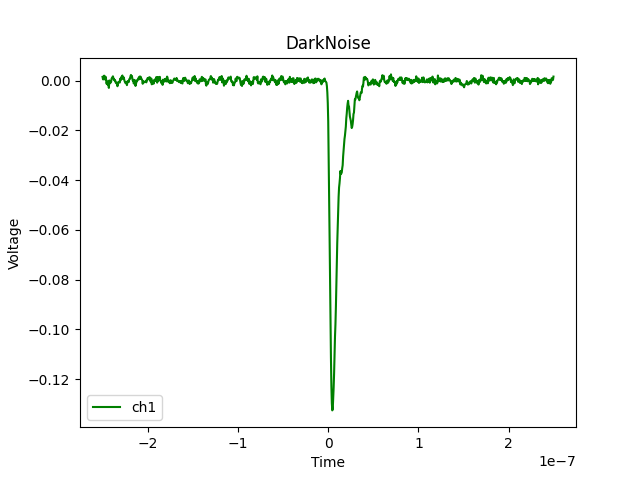
\includegraphics[width=0.5\textwidth]{../AttenuationLength/figs/DarkNoise.png}
\caption{暗噪声,根据一组测量数据作图。}
\end{figure}

通过示波器的频率显示,测量并取平均,得到暗噪声计数率\(n_d \approx \qty{16.02}{s^{-1}}\).
\end{frame}

\begin{frame}[label={sec:org7d2cd88}]{电子学噪声测量}
\begin{figure}[htbp]
\centering
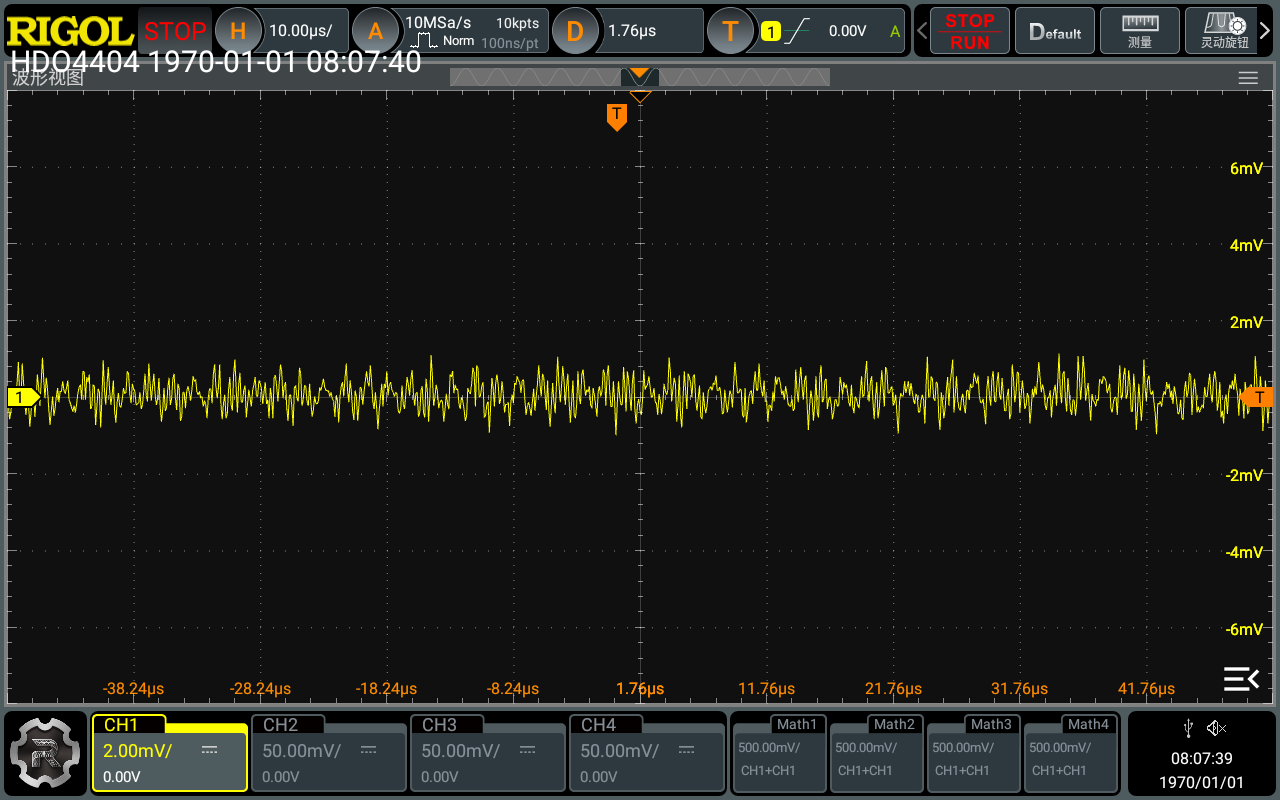
\includegraphics[width=0.6\textwidth]{../ExperimentData/figs/elenoise0.png}
\caption{电子学噪声。}
\end{figure}
\end{frame}
\begin{frame}[label={sec:org9e0e478}]{\(\mu\)子信号测量}
\begin{figure}[htbp]
\centering
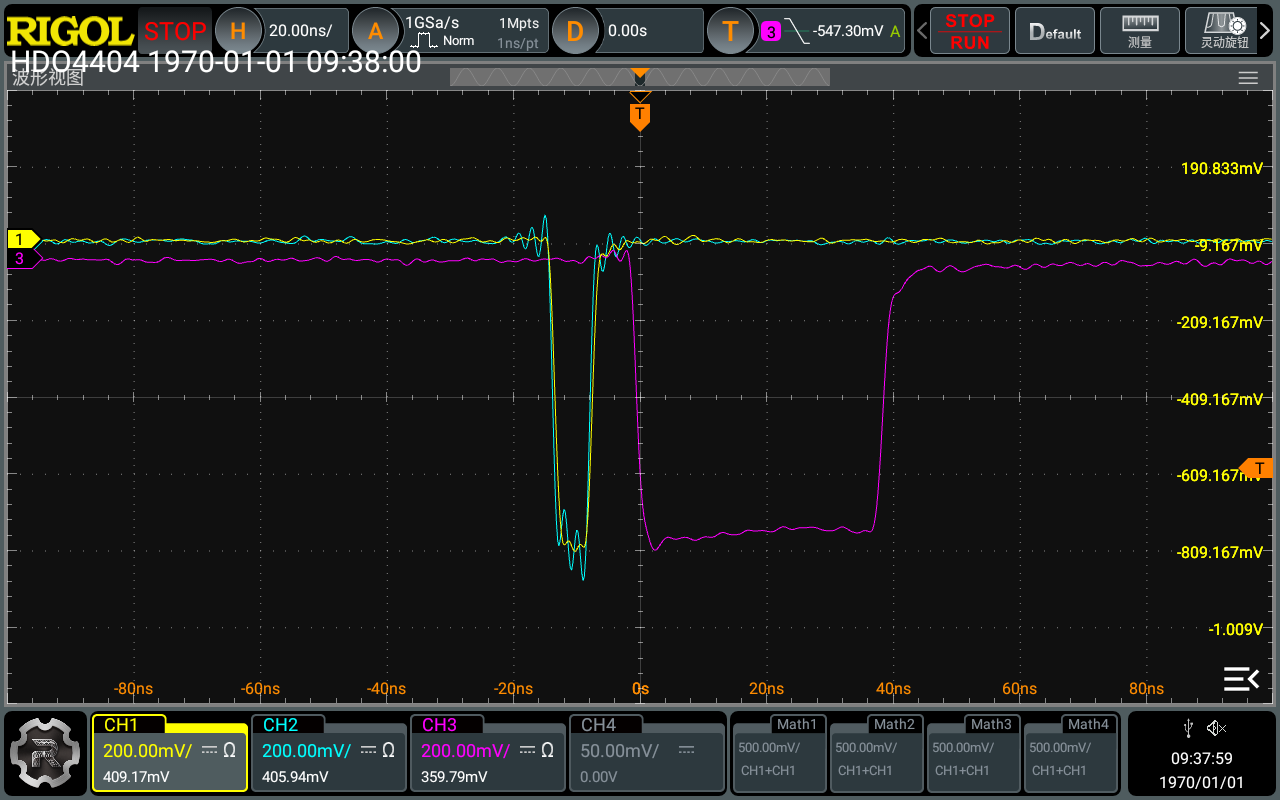
\includegraphics[width=0.6\textwidth]{../ExperimentData/figs/musignal0.png}
\caption{\(\mu\)子信号。}
\end{figure}

测量得到信号计数率 \(n_s \approx \qty{9.98}{s^{-1}}\).
\end{frame}
\begin{frame}[label={sec:org830efa8}]{闪烁光衰减长度测量}
我们知道,光在闪烁体中传播时按指数衰减:
\begin{equation}
\label{eq:1}
q = Q_0 e^{-\frac{L}{L_0}},
\end{equation}
其中\(Q_0\)为初始光子数,\(q\)为传播距离\(L\)后的光子数,\(L_0\)是闪烁体的光衰减长度。

为测量\(L_0\), 我们对闪烁体两端的光信号作符合测量,分别得到两端信号的触发时间和幅度,进而确定信号的时间差和电荷量之比。

由上推导得到:
\begin{equation}
\label{eq:2}
\ln \frac{q_1}{q_2} = -\frac{c}{nL_0}(t_1 - t_2+\Delta t_E),
\end{equation}
其中\(n=1.583\). 进而可通过线性拟合实现衰减长度的测量。
\end{frame}

\begin{frame}[label={sec:orgecbe44e}]{闪烁光衰减后信号符合波形}
\begin{columns}
\begin{column}{0.5\columnwidth}
\begin{figure}[htbp]
\centering
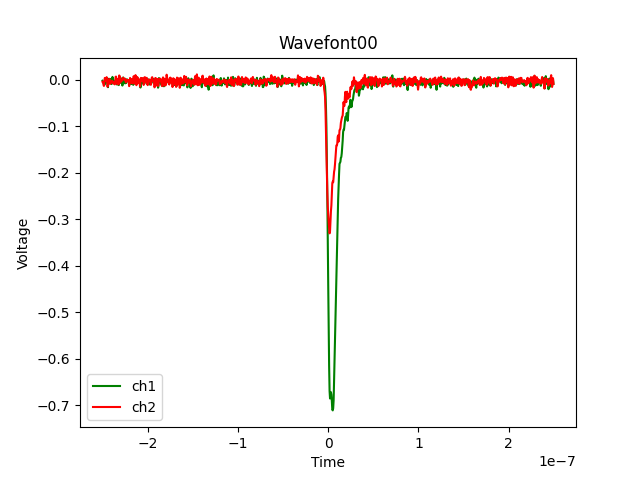
\includegraphics[width=\textwidth]{../AttenuationLength/figs/Wavefont00.png}
\caption{Wavefont00.}
\end{figure}
\end{column}
\begin{column}{0.5\columnwidth}
\begin{figure}[htbp]
\centering
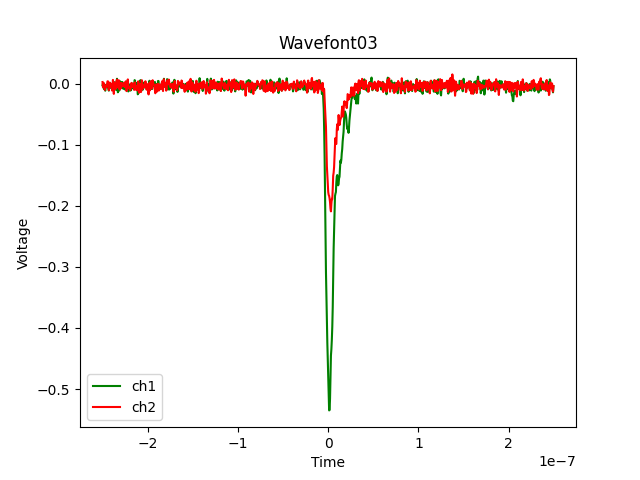
\includegraphics[width=\textwidth]{../AttenuationLength/figs/Wavefont03.png}
\caption{Wavefont03.}
\end{figure}
\end{column}
\end{columns}
\end{frame}

\section{结果分析}
\label{sec:orgc25006c}
\begin{frame}[label={sec:org93946de}]{电荷比值与时间分布}
\begin{figure}[htbp]
\centering
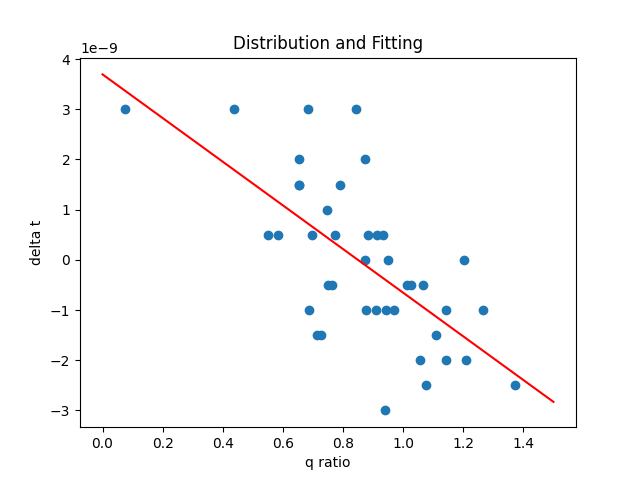
\includegraphics[width=0.4\textwidth]{../AttenuationLength/figs/dist.png}
\caption{电荷比值的自然对数与时间差的分布,以及线性拟合结果。}
\end{figure}

根据拟合结果可计算得
\begin{equation}
\label{eq:3}
L_0 \approx \qty{0.83}{m}.
\end{equation}

线性拟合相关系数 \(R^2 \approx 0.442\), 相对统计不确定度为 0.180.
\end{frame}

\begin{frame}{系统不确定度}
    考虑系统不确定度,主要分为荧光光子衰减,光电子倍增,示波器的时间分辨与电压分辨率几部分:

    忽略光电子倍增与电荷分辨的不确定度,光子衰减的相对不确定度为

    \begin{equation}
    \label{eq:4}
    \sigma_\mathrm{photon}=\sqrt{\frac{2p_1(1-p_1)}{N}+\frac{2p_2(1-p_2)}{N}},
    \end{equation}
    其中$p_1,p_2$分别为两端的光子幸存率,$N$为事例产生的总光子数。
    
    假设总光子数 100,估计相对不确定度为 0.100。

    示波器的时间分辨率为$\Delta t=0.5\mathrm{ns}$,将时间分布视为均匀分布,时间差的不确定度为 $\frac{\Delta t}{\sqrt{6}}$.

    对应的相对不确定度为$\sigma_t=\frac{\Delta tc}{\sqrt{6}nL_0}=0.047.$

    最终得到衰减长度为$0.83\pm0.09_{\mathrm{sysm}}\pm0.15_{\mathrm{stat}}.$
\end{frame}
\section{参考文献}
\label{sec:orgf6ca842}
\begin{frame}[allowframebreaks]{参考文献}
\bibliographystyle{abbrv} % tiny is not good
\bibliography{reference.bib} % 参考文献存放在 "./reference.bib"
\end{frame}
\end{document}
